\documentclass{article}

\usepackage{graphicx}

\setlength{\parskip}{\medskipamount}

\title{Advanced Object Oriented Programming and Design\\
\medskip
\large Theoretical Homework 1}
\author{Abraham Murciano and Daniel Klein}

\begin{document}

\maketitle

\section*{Part 1: Interface Definition}

We are given the following code which we can assume is correct.

\begin{verbatim}
	public static void main(String[] args) {
	    int x;
	    String y;
	    C b1 = new B();
	    A[] arrA = new A[3];
	    arrA[0] = new B(x, y);
	    arrA[1] = new B();
	    arrA[2] = new C();
	    arrA[0].f();
	    arrA[0].g();
	    arrA[0].h();
	}
\end{verbatim}

\subsection*{Section A}

We are told A is an interface, and we are tasked with writing its declaration.

\begin{verbatim}
	interface A {
	    void f();
	    void g();
	    void h();
	}
\end{verbatim}

\subsection*{Section B}

We must now implement classes B and C.

\begin{verbatim}
	class C implements A {
	    void f() {}
	    void g() {}
	    void h() {}
	}

	class B extends C {
	    public B() {}
	    public B(int, String) {}
	}
\end{verbatim}

\subsection*{Section C}

Below is a UML diagram for the classes A, B, and C.

\begin{figure}[htbp]
	\centering
	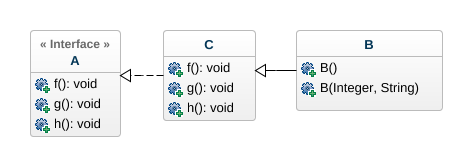
\includegraphics[width=\textwidth]{uml.png}
\end{figure}


\subsection*{Section D}

C cannot be an interface, because we call its constructor in the code, and interfaces cannot be instantiated.

\section*{Part 2: Plane and Train System}

If our plane and train classes would implement the \verb`Comparable` interface, then when calling \verb`sortTarnsport` on an array containing both of these different types, we would get an error saying that we cannot cast from one of the types to the other. However, if these classes implement the generic \verb`Comparable<T>` interface, where \verb`T` is the class \verb`Train` or \verb`Plane`, then our code would not allow for such a circumstance to occur, since we must pass it specifically an array of \verb`Train` objects or \verb`Plane` objects, not anything else.

\end{document}